\section*{Reciprocity \& Network Effects}
\label{neteffects}

In studies of social and economic behavior, direct reciprocity--the notion that actors tend to ``respond in kind" to one another--is argued to be an essential component of human behavior (For example, see \cite{bolton:1998, charness:2002, charness:2004, cox:2007, cox:2004}.). The idea that individuals, or collectives, observe previously cooperative (or conflictual) behavior from others, and include this information into their own decision-making is a concept given great value to determine strategic outcomes. For example, reciprocity has been showed to influence  interactions across diverse settings including tax compliance \citep{smith:1990}, wage selection \citep{campbell:1997}, and strike breaking \citep{brett:1998}. Reciprocity is also shown to play a critical role in the development of interethnic attitudes whereby groups tend to reflect the attitudes that other groups hold toward them.\citep{berry:1979}. %last sentence too abrupt? 

International relations scholars have also long argued that reciprocity is critical to the evolution of cooperative and conflictual interactions among states. This assertion dates back to early research on foreign policy. Scholars concerned with understanding the onset of World War I acknowledged the importance of tit-for-tat interactions \citep{holsti1972}. This same logic is rooted in research investigating the prisoner's dilemma. \cite{axelrod:1985} outlines the basic logic of reactive response in repeated interactions and highlights how reciprocal interactions over time foster cooperation. \cite{rajmaira:1990} find that reciprocity determines long-term foreign policy behavior among superpowers. In other realms of international politics, reciprocity plays a key role in formulating expectations of state behavior. Take, for example, the theoretical weight of reciprocity in the literature on international laws of war; a literature which has been traditionally assessed whether one state will ``respond in kind" to another state's treatment of prisoners, soldiers, and civilians during wartime. As one scholar notes, ``It is an empirical datum that people tend to respond to others with an implicit policy of like for like and that this facilitates cooperation between them. This elementary fact has profound implications for the effective design of law and institutions.'' \cite[p. 19]{osiel:2009}. Why then have current theoretical accounts of international sanctions ignored the role of reciprocity? 

We argue that reciprocity influences sanction outcomes through two key processes: behavioral expectations and information sharing. The first process is that which is promoted by existing work on reciprocity and cooperation: one actor has incentive to ``respond in kind'' to the previous behavior of their partner. In international relations, states that are perceived as cooperative will be more likely to have future partners cooperate with them.
%probably need to add the surprising "sanctions are not one directional" here?
The sanctioning process has also been conceptualized as form of international bargaining (Morgan and Miers 1999, Marinov 2002, Lacy and Niou 2004). In any sanction case, there is uncertainty about the target state's willingness and capacity to endure the sanction.  Any time a sanction is endured information is shared between states as both the sender and target state decide how to respond to one another's behavior. During this time, each state reveals more information about their preferences and resolve.  We argue that the evolution of ties between sender and target states influences the calculation states make over time through revealing previously unknown preferences for cooperation. The two explanations that we focus on are (1) reciprocity in the sanctioning network over time; (2) previous compliance reciprocity.\footnote{``Sender'' states are those that impose or threaten sanctions, while ``receiver'' states are those that states in which sanctions are imposed.}

\begin{figure}[ht]
  \centering
  \begin{tabular}{c}
	  \includegraphics[width=1\textwidth]{84net-crop} \\
	  \includegraphics[width=0.45\textwidth]{MapLegend}
  \end{tabular}
  \caption{Here we show the sanction network in 1984, nodes are colored by geographic coordinates of countries. Data for sanction cases comes from \citet{morgan2009threat}.}
  \label{fig:spaghetti}
\end{figure}
\FloatBarrier

To demonstrate these two forms of reciprocity, we visually present the sanction-year network. Figure \ref{fig:spaghetti} depicts the network of sanction cases on-going and initiated by 1984. This network graph presents the entire sanction-year network.  Nodes represent states and the directed edges denote the sender and receiver of sanctions. This figure is complex, showing that each yearly network contains important information about state behavior, whereby numerous states are involved in multiple sanction cases during this individual year. Typical analysis on sanction duration does not capture sanction-year attributes and ignores how these network characteristics evolve over-time to inform future behavior within sanction networks. While studies of international relations tend to recognize the interdependent nature of state behavior in the theoretical sense, they often fail to uphold this theoretical intuition in empirical analysis. Early attempts are noteworthy,\footnote{\cite{keohane1989reciprocity,goldstein1991reciprocity}} and more recent work has continued to address this concern,\footnote{\cite{mitchell2001,cranmer2014reciprocity}} yet studies on sanction compliance have not yet incorporated these insights. 

We develop two reciprocity concepts that allow us to analyze the interdependencies inherent to the evolution of sanction dynamics. First, we outline a \textit{compliance reciprocity} measure. By creating a yearly network, for each year available in our data, we are able to calculate compliance reciprocity over time. Essentially, this represents a target states' cumulative history of compliance with a particular sender relative to all others in the network. This can be thought of as a record of compliance between an individual dyad pair, relative to all other dyads within the network. 

 Our measure of reciprocity allows us to capture whether those who have a history of cooperative behavior with each other also tend to have more cooperative behavior in the future with partner states. In a duration context, states who receive sanctions from those with whom they have a history of reciprocal compliance are likely to comply sooner to those states than they would with lower compliance reciprocity. Notably, this measure is different from a simple conceptualization of past interactions which might simply control for the number of times a state has complied. Such a simple measure completely ignores the fact that each state's actions are conditional on all other interactions between states. For example, if state $i$ complies often to state $j$, is state $i$ also more likely to comply with all other partner states? Or, relative to all other interactions, does state $i$ comply more frequently and uniquely with state $j$? The latter idea is the one explicated within our  concept of compliance reciprocity. Thus, reciprocity tells us information about the interactions between country $i$ and $j$ over time, relative to how country $i$ interacts with all other partners over time. 

% The majority of studies on sanctions treat all sanctions cases, as well as sanction actors, as independent from other another. Because multiple actors appear within multiple sanction cases in any given year, (i.e. the USA might act as a sender state against South Africa in several different economic sanction cases within one year), our approach allows for us to directly address the interdependencies both between sanction cases as between sanction senders. 

We draw our measure of reciprocity from the Social Relations Model developed by \citet{kenny1994interpersonal} and presented as a tool for political scientists by \cite{AnneAuthor}. To illustrate, consider the matrix $X_{ij}$ below, in which we have six actors in a round robin (dyadic) format. These data are represented by the matrix below, which has the value for each of the thirty interactions, with the main diagonal remaining empty:

\singlespacing
\[
\left[
\begin{array}{cccccc}
 & X_{12}  & X_{13}  & X_{14} & X_{15} & X_{16} \\
X_{21}  &  & X_{23}  & X_{24} & X_{25} & X_{26} \\
X_{31}  & X_{32}  &    & X_{34} & X_{35} & X_{36} \\
X_{41}  & X_{42}  & X_{43}  &  & X_{45} & X_{46} \\
X_{51}  & X_{52}  & X_{53}  & X_{54} &   & X_{56} \\
X_{61}  & X_{62}  & X_{63}  & X_{64} & X_{65} &   \\
\end{array}
\right]
\]

\doublespacing
First, we begin with calculating the row column and total sums:
\begin{itemize}
\item The totals for each \emph{ row} are denoted $X_{i \cdot}$ where $i$ is the row number, i.e.,
~\\
$X_{i \cdot} = \sum_{j=1}^{J} X_{ij}$;
\item For each column the totals are denoted
 $X_{\cdot i}$ where $i$ is the \emph{column} number; and 
 \item The total over all rows and columns is given by $X_{\cdot \cdot} = \sum_i \sum_j X_{i,j}$.
 \end{itemize}
 
Given these quantities, one can calculate individual effects for a variety of concepts, such as the actor, partner, and unique dyadic effects, (as well as the variances attributed to each of these effects). The unique dyadic effects, or the reciprocal interactions between two countries within one pair, are calculated accounting for the general behavior of each country within the pair. Or, in other words, this measure captures how likely country $i$ is to comply with country $j$; and the likelihood that country $j$ is to comply with country $i$ is calculated relative to how often country $i$ tends to comply with all of the other countries, as well as how likely country $j$ is to comply to all others. 

 \begin{itemize}
 \item The actor effect for observation $i$ is the total of $i$'s row mean and column mean, minus the overall mean.  The means are just the sums, corrected for degrees of freedom, yielding an average row effect:\\
 $\hat{a}_i = \frac{(n-1)^2}{n(n-2)} X_{i \cdot} + \frac{(n-1)}{n(n-2)} X_{\cdot i} -  \frac{n-1}{n-2} X_{\cdot \cdot} $
\item Similarly the column mean for actor $i$ is \\
 $\hat{b}_i = \frac{(n-1)^2}{n(n-2)} X_{\cdot i} + \frac{(n-1)}{n(n-2)} X_{i \cdot } -  \frac{n-1}{n-2} X_{\cdot \cdot} $.\\ For a symmetric matrix, the row effect and the column effect will be identical.
\item The unique dyadic effect, or reciprocity for specific dyad $ij$, simply subtracts the row and column effects along with the overall mean out of the value for dyad $ij$. \\
$\hat{g}_{ij} = X_{ij} - \hat{a}_i - \hat{b}_j - X_{\cdot \cdot}$
 \end{itemize}

\doublespacing
The first two equations show how the final equation for reciprocity is calculated relative to the general actor and partner effects (or actor and partner average behavior) for each country.\footnote{\cite{kenny1994interpersonal} would suggest including the full compliment of the SRM into our model. We originally explored this approach, but gained little empirical leverage from it, and thus focus instead on the concept of reciprocity.} %CD: should this be a footnote

We extend this intuition to our second key measure, \textit{sanction reciprocity}. Following the same idea as compliance reciprocity, this is a measure of how often a target state has received sanctions from the senders of any given sanction case--relative to all other sanction interactions of states. The intuition behind this measure is to capture the concept of resolve: states who have been sanctioned multiple times by a sender state are likely to build up a willingness of resistance and not cooperation.  This suggests that states receiving sanctions from those with whom they have been sanctioned before are likely to more slowly comply to those states. 

\begin{figure}[ht]
	\centering
	\caption{Reciprocity plots}
	\begin{tabular}{ccc}

	\subfloat[sub1][Compliance: 1972]{
		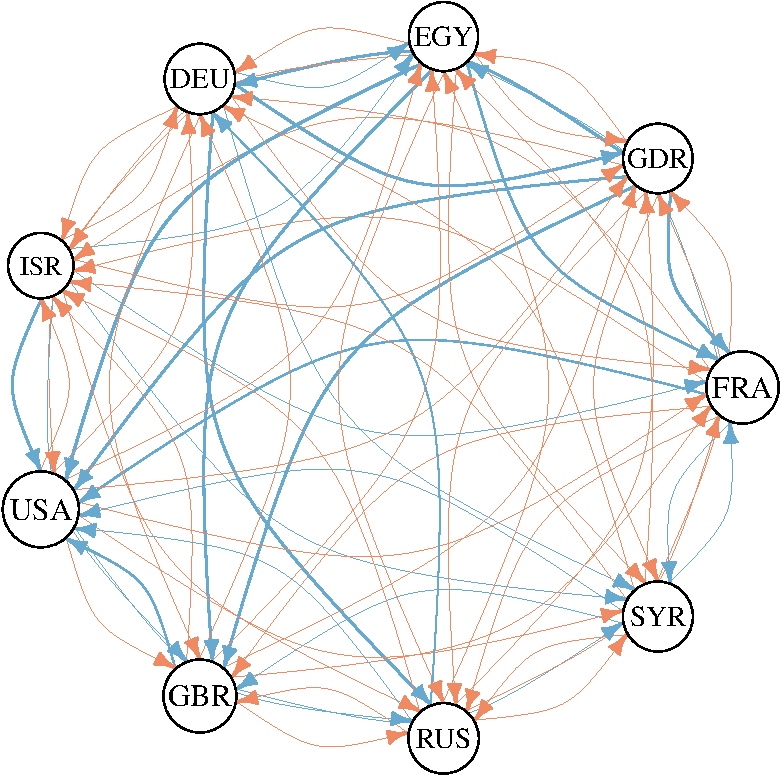
\includegraphics[width=.33\textwidth]{compNet_1972}
		\label{fig:comp72}} & 

	\subfloat[sub1][Compliance: 1992]{
		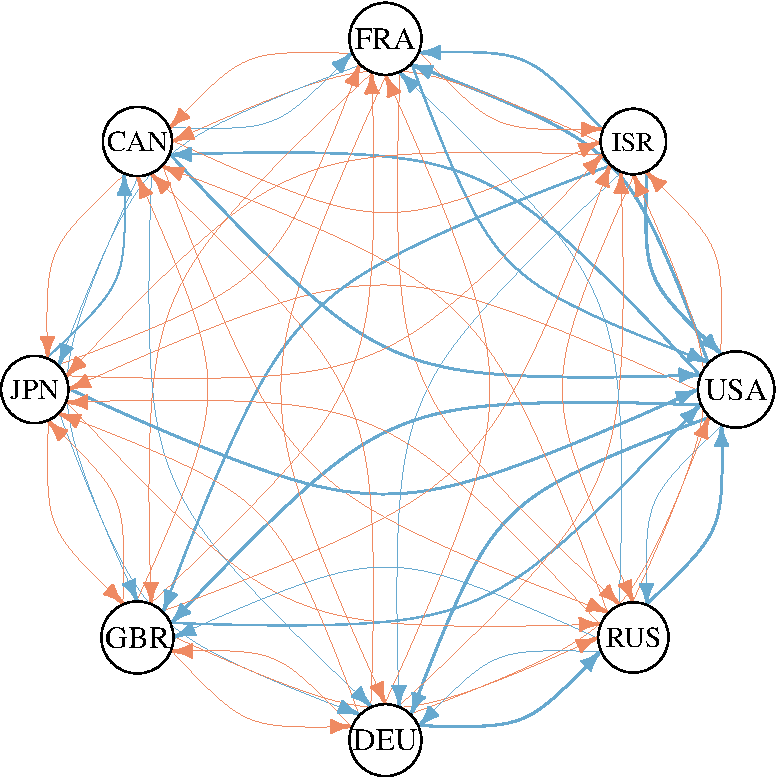
\includegraphics[width=.33\textwidth]{compNet_1992}
		\label{fig:comp92}} & 

	\subfloat[sub1][Compliance: 2012]{
		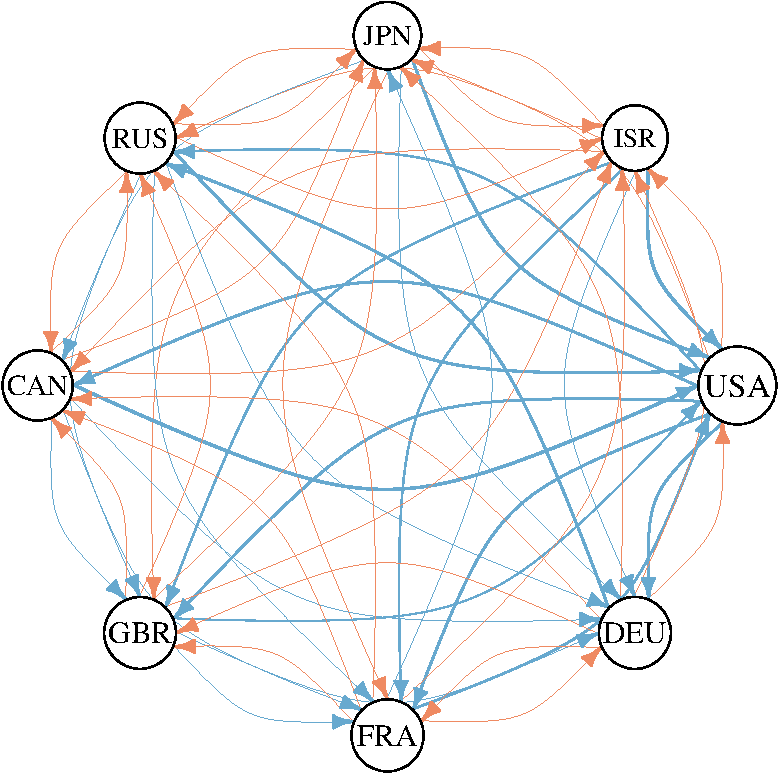
\includegraphics[width=.33\textwidth]{compNet_2012}
		\label{fig:comp02}} \\

	\subfloat[sub1][Sanction: 1972]{
		\includegraphics[width=.33\textwidth]{sancNet_1972}
		\label{fig:sanc72}} & 

	\subfloat[sub1][Sanction: 1992]{
		\includegraphics[width=.33\textwidth]{sancNet_1992}
		\label{fig:sanc92}} & 

	\subfloat[sub1][Sanction: 2012]{
		\includegraphics[width=.33\textwidth]{sancNet_2012}
		\label{fig:sanc02}}

	\end{tabular}
	\label{fig:recipNet}
\end{figure}

The basic insight here is that those states which continually reciprocate sanctioning behavior are signaling more conflictual behavior rather than cooperative behavior. 

\begin{quote}
	\textbf{H1}: states who receive sanctions from senders they have a history of reciprocal compliance are likely to comply quickly. 
\end{quote}

\begin{quote}
	\textbf{H2}: states receiving sanctions from those with whom they have a history of higher sanction reciprocity will be slower to comply.
\end{quote}

%We also account for key conditions at the sanction-case level. To demonstrate, we deconstruct the broader yearly network example of 1984, to zoom in and narrow our focus to observe the individual sanction case of South Africa in 1984. In this case, South Africa is the target of multiple sanctions, as shown in Figure \ref{fig:saneti}. Because of this, we construct a sanction network that represents each sanction South Africa faces during this year. As one can easily see, in most cases during 1984, South Africa faces more than one sanctioner, and these sanctioners vary across each sanction case. For example in the first network graph, in the top left of Figure \ref{fig:saneti}, we see that South Africa faces a sanction from India, Pakistan, and Jamaica. Yet in the top right network graph, we see that South Africa also faces a sanction from Canada, Sweden, the USA, Finland, and Australia. 
%
%By the 1980s, the South African apartheid regime had been in power for over thirty years. The international community moved to sanction the apartheid regime in hopes to end the violence and delegitimize the regime. As unrest intensified international action became inevitable and multilateral economic sanctions were initiated. As \citet{kinne2013dependent} points out, the aim of delegitimizing a regime is a cooperative act between multiple actors, whereby its effectiveness is dependent on coordinated consent and action. To diplomatically exclude South Africa, successful coordination and cooperation amongst sanctioner states was key.\footnote{\cite{kinne2013dependent,christopher1994pattern}} Critical coordination was achieved through this group of state sanctioners. By also looking at the sanction-case network, we are able to capture these state-level to test whether characteristics among sanctioners effect sanction compliance. For example, we might expect that a sanction from Pakistan, India, and Jamaica has substantially different implications than one from largely ``western'' sanctioners such as Sweden, Canada, USA, Finland and Australia. We conceptualize these relationships as composed of ``pressures'' which likely influences the behavior of the target state. We present two hypotheses which focus on the sanction case network. First, it is intuitive that the number of senders should influence the willingness of the target state to comply because as the number of senders increases, the more constraints through multiple relationships the target faces. 
%\begin{figure}[ht]
%	\centering
%	\includegraphics[width=1\textwidth]{saneti}
%	\caption{Network for each sanction case that South Africa faced in 1984.}
%	\label{fig:saneti}
%\end{figure}
%\FloatBarrier
%
%We also expect that these relationships must be meaningful not just plentiful. Just as one would imagine that a person is less swayed by the demands of 10 strangers than the demands of a few close friends, we conceptualize senders as most influential when they interact with the target state on a number of dimensions.  Thus, for each sanction case we determine the number of senders but we also measure other dimensions of each sender's relationship to the target. In addition, we calculate and control for the average number of other sanctions being sent by the senders of each particular sanction case.
%
%\begin{quote}
%	\textbf{H3}: As the number of sender states increases for any given sanction case, the time to compliance will decrease. 
%\end{quote}
%
% We now describe exactly what is meant behind our concept of ``proximity.'' In figure \ref{fig:saneti}, we show the six sanction cases faced by South Africa in 1984.\footnote{Data for sanction cases are from \citet{morgan2009threat} and is explained further in the following section.} For the most part, each sanction case involves a variety of actors with whom South Africa has differing cultural, geographic, diplomatic, and economic relationships. Within any individual sanction case we hypothesize (\textbf{H4}) that the proximity, (i.e. the ways in which the sender and target interact on a number of dimensions) of relationships between sender(s) of a sanction and a receiver influence whether a target state complies. We construct a number of covariates to test this idea that the normative closeness, or general ``proximity'' between sender(s) and receiver(s) increases sanction compliance. 
%
%We focus on five key measures of the ``proximate'' nature of relationships. First, we measure the average distance between sender(s) and receiver.\footnote{To construct this measure we use the minimum distance between countries from the Cshapes Dataset \citep{weidmann2010geography}.} We utilize the Correlates of War (COW) data to construct the remaining four variables. Our second covariate relating to proximity is trade, which we measure as the total share of the receiver's trade in that year accounted for by sender states. Last, we measure alliances as the proportion of sender(s) that are allied with the receiver. 
%
%\begin{quote}
%	\textbf{H4}: Sanction cases where relationships between sender(s) and receiver(s) are more proximate will be more quickly resolved.
%\end{quote}
%
%%%%%%%
%% SM NOTE: commented this out for now since we dont include this variable in the current set of models. also it doesnt load in the current set of models. i'm thinking that we might just want to dump this hypothesis and the corresponding figure (which i think you had suggested already).
%
%% Thus far we have explained how the relationships between sanctioners and target states matter for predicting compliance. This view has focused on the individual sanction case. However, the six separate sanctions that South Africa faced in 1984 can also be thought of within the context of a yearly sanction network. In figure \ref{fig:sanet}, we aggregate the six sanction networks into one where each separate sanction is denoted by a differing color. Here we hypothesize that states under the pressure of a multitude of sanctions will more quickly resolve sanction cases than those facing only a few.
%
%% \begin{quote}
%% 	\textbf{H3}: States facing the pressure of a multitude of sanctions will more quickly resolve any one of those sanction cases.
%% \end{quote}
%
%% \begin{figure}[ht]
%% 	\centering
%% 	\includegraphics[width=0.75\textwidth]{sanet}
%% 	\caption{All sanctions faced by South Africa in 1984 collapsed to one network}
%% 	\label{fig:sanet}
%% \end{figure}
%% \FloatBarrier
%%%%%%%%%
%
%Last, we include a number of covariates to account for domestic explanations of sanction compliance in the extant literature. First is a measure of the target states' domestic institutions from the Polity IV data.\footnote{See \cite{marshall2002polity}. Specifically, we use the ``polity2'' variable from the Polity IV data.} This measure is computed by subtracting a country's autocracy score from its democracy score, and is scaled from 0 to 20. Previous research has shown that sanctions will be more effective when the target states' domestic institutions are more democratic. Second, we control for the level of internal conflict within  a country using the weighted conflict index from the Cross National Time-series Data Archive.\footnote{\cite{banks2011cross}} The expectation in the extant literature is that countries with higher levels of internal instability would be more likely to comply to sanctions. Finally, we use a logged measure of GDP per capita and the percent change in annual GDP, from the World Bank, to account for the argument that economically successful states are better able to weather the pressures of these agreements.